\setAuthor{Päivo Simson}
\setRound{lahtine}
\setYear{2023}
\setNumber{G 4}
\setDifficulty{4}
\setTopic{TODO}

\prob{Kondensaatorid}
\begin{wrapfigure}{r}{0.19\textwidth}
\vspace{-0.8cm}
  \begin{center}
    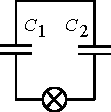
\includegraphics[width=1\linewidth]{2023-lahg-04-yl.pdf}
    %\caption{}
  \end{center}
  \vspace{-0.9cm}
\end{wrapfigure}

Indrekul on kaks kondensaatorit mahtuvustega $C_1=40\,\mu$F ja $C_2=60\,\mu$F. Esimene neist ($C_1$) on laetud pingeni $U_0$ = 15 kV ja teine ($C_2$) on pingeta. Indrek soovib teist kondensaatorit esimese abil laadida, aga kardab, et laadimisjuhtmed süttivad suure voolutugevuse tõttu. Selle vältimiseks lisab ta ahelasse hõõglambi (vt joonis). Kui suur soojushulk eraldub  kogu süsteemis, kui Indrek hoiab kondensaatoreid ühenduses pikka aega?






\hint

\solu
Enne laadimise algust on esimese kondensaatori energia
\[E_1=\frac{C_1U_0^2}{2}=4500\,\textrm{J}\]
ja teise energia on null. Laadimise käigus toimub kondensaatorite vahel laengu ümberjaotumine, kuid kogulaeng $q$ säilib. Laadimisprotsess toimub seni, kuni kondensaatorite pinged võrdsustuvad. Lõpp-pinge $U$ saame leida laengu jäävuse seadusest:
\[q=C_1U_0=C_1U+C_2U\quad\implies\quad U=\frac{C_1U_0}{C_1+C_2}=6\,\textrm{kV}.\]
Laadimise lõpuks on kahe kondensaatori koguenergia
\[E_2=\frac{C_1U^2}{2}+\frac{C_2U^2}{2}=\frac{(C_1+C_2)U^2}{2}=1800\,\textrm{J}.\]
Näeme, et see on väiksem kui esimese kondensaatori energia enne laadimise algust. Puuduolev energia eraldus järelikult süsteemist soojusena, peamiselt hõõglambi põlemisel. Otsitav soojushulk on seega
\[Q=E_1-E_2=2700\,\textrm{J}.\]
\emph{Märkus:} ülesande võib lahendada ka vahetulemusi kasutamata. Energia ja laengu jäävustest saame
\[
\begin{cases}
\displaystyle\frac{C_1U_0^2}{2}=\frac{C_1U^2}{2}+\frac{C_2U^2}{2}+Q\\
\,\,C_1U_0=C_1U+C_2U
\end{cases}
\implies Q=\frac{C_1C_2U_0^2}{2(C_1+C_2)}=2700\,\textrm{J}.
\]
\probend